\documentclass[a4paper, 12pt]{article}

\usepackage[utf8]{inputenc}
\usepackage[T1]{fontenc}
\usepackage[margin=0.5in]{geometry}
\usepackage{graphicx}
\usepackage[font={footnotesize,it}]{caption}
\usepackage{hyperref}

\begin{document}

\setlength{\parindent}{0pt}

\title{Guía para el uso de Git en Linux\\
\large Algoritmos y Programación I}
\author{Julián García Delfino}
\maketitle
\newpage
	  
\tableofcontents
\newpage

\section{Introducción a Git}

\subsection{¿Qué es Git?}

\begin{description}
\item[Git] Es un software de control de versiones que se usa para poder hacer un correcto seguimiento al desarrollo de programas que tienen archivos extensos que contienen sus códigos.
\end{description}

Y entonces, ¿Cómo funciona?

\subsubsection{Definiciones que nos pueden ayudar}

\begin{description}
\item[Repositorio] En sistemas de revisión de versiones, como Git, un repositorio es una estructura de datos que guarda \textbf{metadata} de un conjunto de archivos.
\item[Metadata] Es informacion sobre nuestros archivos. \textit{"Data that provides information about other data"}
\end{description}

\subsubsection{Idea general del funcionamiento}

Con la información que tenemos hasta ahora, podríamos esbozar, en el aire, una idea de cómo funciona Git.\\
Al crear un repositorio, estamos habilitando al sistema de revisión de versiones a que guarde cierta información sobre los archivos que nosotros pongamos en ese directorio. Es decir, si tenemos nuestro código con extensión, por ejemplo, \textbf{.c} en una carpeta que a la vez es un repo de Git, éste puede, gracias a la metadata que almacena, llevar la cuenta de los cambios que se generan entre versiones del programa.\\
Esto podría ser muy conveniente si estamos trabajando en algo muy complejo, o incluso sólamente extenso.

\subsection{Funcionamiento de Git}

Entonces, ya generamos una idea sobre qué es lo que hace Git con nuestros datos, pero puede ser que todavía sea muy vaga y abstracta.\\

Básicamente, nuestra información se moverá entre 3 etapas:

\begin{itemize}
\item Working Directory
\item Staging Area
\item Repository
\end{itemize}

\subsubsection{Working Directory}
El \textbf{Working Directory} es, básicamente, donde tendremos almacenados los archivos sobre los que trabajaremos y donde luego, también, crearemos el repositorio de Git.\\
Por ejemplo:

\begin{verbatim}
        $ sudo mkdir proyecto1 /*Creo la carpeta donde almacenaré los archivos*/
        $ cd proyecto1 /*Me muevo dentro de esa carpeta*/
        $ git init
        Initialized empty Git repository in /direcciónPrevia/proyecto1/.git
\end{verbatim} 

Ahora \textbf{proyecto1} es mi \textbf{Working Directory}.

\subsubsection{Staging Area}
El \textbf{Staging Area} es la etapa donde vamos a preparar el \textbf{commit}, o por ahora, la \textbf{entrega}.\\

Como veremos mejor mas adelante, no basta con realizar cambios a los archivos, sino que hay que \textit{"agregarlos"} al \textbf{Staging Area}.\\
Imagínense que estamos haciendo el trabajo práctico de la materia, pero, antes de seguir avanzando queremos ir llevando la cuenta de los cambios importantes que le hacemos a nuestros archivos. Entonces, tenemos creada la carpeta, el \textit{Working Directory}, y dentro de ella inicializamos el repo de Git. Ya hicimos cambios y queremos asentarlos.\\
Git, a esta altura, sabe todas las modificaciones que se fueron haciendo en el tiempo, desde la creación del repositorio, pero hasta que no las agregamos al \textbf{Staging Area}, éste no podrá hacer nada con esta información.\\
Entonces, agregamos todos los archivos que querramos entregar y formamos un \textit{paquete} con estos.
El \textbf{Staging Area} se encarga de eso, de ser el paquete que entregaremos con toda la información que necesita Git para seguir el rasto.

\subsubsection{Repository}
El \textbf{Repositorio} es donde Git almacenará toda la metadata que necesita para generar el registro de control de versiones.\\

Entonces, tenemos el paquete armado en el \textit{Staging Area} y queremos mandarlo al \textbf{repositorio}, basta hacer el \textit{commit} y listo. Git tendrá toda la información que necesita.
Pero, ¿Cómo sabemos nosotros qué cosas se cambiaron concretamente?
Bueno, con cada \textit{commit} se debe poner un mensaje que especifique de forma clara qué cosas se cambiaron.\\

Por ejemplo:

\begin{verbatim}
 "Implementación de la función de suma"
                   ^
                   |
                Commit
     |Paquete| -------> |Repositorio|
\end{verbatim}

\section*{Panorama General}
Ahora, ya tenemos todas las piezas del rompecabezas que es el funcionamiento de Git.\\ Si lo pusiésemos todo junto nos quedaría algo así:\\

\begin{figure}[h!]
\centering
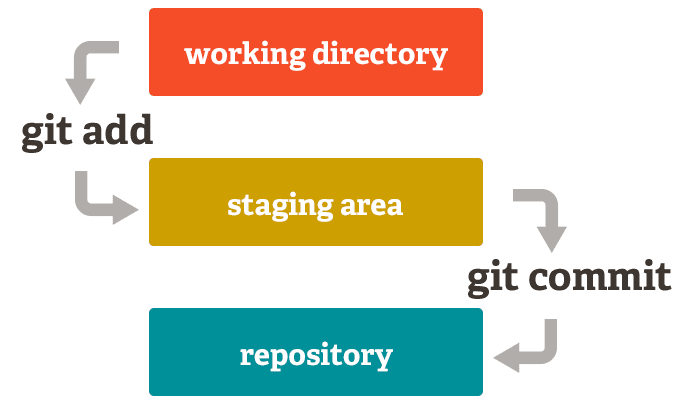
\includegraphics[scale=0.35]{panoramaGen.png}
\caption{\small Esquema del funcionamiento de Git.}
\end{figure}

\newpage

\section{Instalación de Git}

En el cmd (Ctrl + Alt + t):\\

\verb+        $ sudo apt install git-all+\\

Obs: Este comando funciona para distros basados en Debian (Como Ubuntu).

\subsection{Configuración Opcional}

Hay algunas cosas más que podemos configurar de Git que podrían, en algún momento, sernos útiles.\\

\verb+        $ git config --global user.name "Tony Stank"+\\

Ésto lo que hace es, configurar un estilo de sello que irá en cada paquete que se commitée a Git.\\

\verb+        $ git config --global user.email "direcciónDeCorreo@Algoritmos1.com"+\\

Acá, a ese sello, le agregamos nuestro mail. Puede ser que no les parezca algo que pueden llegar a usar ahora, y tienen razón. Éste es, capaz, un aspecto de Git que puede ser muy útil en proyectos más grandes, con más personas. Si alguno de sus integrantes necesita contactarse con la persona que hizo un commit específico al código, puede hacerlo directamente a esa dirección.

\newpage
\section{Crear un repositorio}

Primero, debemos movernos a la posición dentro de la PC donde querramos inicializar el repo, es decir, donde vamos a guardar nuestro proyecto (Comandos cd y mkdir).\\

Una vez ahí:
    
\begin{verbatim}
        $ mkdir prueba
        $ cd prueba
        $ git init 
        Initialized empty Git repository in /Dirección/.git/ 
\end{verbatim}
    
\subsection{Archivo README}

Es buena costumbre agregar un archivo README para informar exactamente para qué será utilizado el repo:\\

\verb+        $ nano README.txt+\\

Como sabemos, nano es un editor de texto que viene integrado con la consola de linux.\\
Para confirmar que guardaron el archivo correctamente podrían usar el comando:

\begin{verbatim}
        $ ls 
        README.txt
\end{verbatim}

También, existe el comando \texttt{\$ git status} que nos mostrará los cambios hechos en los archivos que hemos indicado que debe seguir. En el siguiente ejemplo, Git nos avisará que hay un archivo, pero no le esta haciendo el seguimiento.

\begin{verbatim}
        $ git status
        On branch master

        No commits yet

        Untracked files:
            (use "git add <file>..." to include in what will be committed)

                README.txt

        nothing added to commit but untracked files present (use "git add" to track)
\end{verbatim}

\newpage

\section{Add y Commit}

Un \textbf{commit} es como un registro de actividades dentro del repo, es decir, una \textit{entrega}. Cada vez que se haga un \textbf{commit}, Git registrará tanto la adición como la modificación de archivos y llevará la cuenta. Ésto es lo que nos facilitará el control de versiones en un futuro.\\

Git detectará los cambios hechos en el repositorio, pero a menos que usemos el comando \texttt{\$ git add <filename>}, éste no hará nada con ellos. Es decir:

\begin{verbatim}
        $ git add README.txt 
        $ git status
        On branch master  

        No commits yet

        Changes to be committed:
                (use "git rm --cached <file>..." to unstage)

                new file:   README.txt
\end{verbatim}

Ahora Git ya conoce nuestro archivo y debemos hacer un \textbf{commit}:\\

\verb+        $ git commit -m "Mensaje descriptivo sobre las modificaciones y adiciones"+\\

Por ejemplo:\\

\verb+        $ git commit -m "Primera subida - README"+

Si hemos hecho cambios en nuestro archivo y no hemos hecho un \textbf{commit} porque decidimos que queremos revertirlos, podemos usar:

\verb+        $ git checkout -- <filename>+\\
\verb+        $ git checkout -- .+\\

Ésto revertirá los cambios por archivo, individualmente, o a todos a la vez.

\section{Branches y Merge}

Supongamos que ahora queremos agregar alguna función nueva al programa pero no queremos, todavía, generar cambios en el proyecto principal. Para esto usamos un \textbf{Branch•}.\\

Para crear un Branch nuevo:\\

\verb+        $ git checkout -b <branchName>+\\

¿Por qué \textbf{checkout}?
Una vez creado el \textbf{Branch}, como queremos trabajar en él, Git nos saca del master branch y nos mueve a esta rama recien creada.\\
Para chequear los branches disponibles podemos usar:\\

\verb+        $ git branch+\\

Siguiendo con nuestor ejemplo:

\begin{verbatim}
        $ git checkout -b "branch1"
        Switched to a new branch 'branch1'
        $ git branch
        * branch1
        master
\end{verbatim}

Para cambiar entre repositorios existentes:\\

\verb+        $ git checkout "existingBranchName"+\\

Los cambios hechos en \textbf{branch1} no afectarán a los commits en el branch principal \textbf{master}. Una vez finalizado el desarrollo en la rama secundaria, se podría mergear el contenido de ambas en la principal:\\

\verb+        $ git merge branch1+

\section{Extra}

\subsection{Comandos Extra}

\subsubsection{Help}

Para ver la documnetación de Git podemos usar:\\

\verb+        $ git help+\\

Y también, individualmente por argumento:\\

\verb+        $ git argumentName --help+\\
\verb+        $ git add --help /*Por ejemplo*/+\\

\subsubsection{Stashing}

El \textbf{Stash} es una herramienta muy útil que nos permite \textit{almacenar} o justamente \textit{stash} en una \textit{repisa} o \textit{shelf}, temporalmente, los cambios hechos en nuestros archivos por branch.\\

En otras palabras, imaginen que estamos trabajando en un \textit{branch != master} que estamos usando para la implementación de una función específica. Por alguna razón, tenemos que cambiar de branch para retomar en otra sección del programa pero no terminamos la implementación en la que estábamos. Una parte de código sin terminar puede traer muchos dolores de cabeza, entonces, es conveniente deshacerse de los cambios que hicimos sin necesariamente perderlos, así en un futuro lo terminamos.\\

Acá es donde entra el stashing. Ilustraré los comandos con un ejemplo simple.\\

Supongamos que estamos implementando un programa que tiene dos funciones, una de suma y una de resta. Como buena costumbre, crearemos un branch para cada función para poder trabajar tranquilamente en ellas por separado.\\

Estando en branch \textit{Suma}, quiero pasar al branch \textit{Resta} pero no quiero perder los cambios en la función de suma:

\begin{verbatim}
        $ git diff /*Nos muestra los cambios que hicimos actualmente*/
        $ git stash save "Implementación de la función suma"
        
        $git stash list /*Lista de stashes almacenados en este branch*/
        stash{0}: On suma: Implementación de la función suma
\end{verbatim}

Nuestros cambios están guardados en un estante virtual, y nosotros podemos seguir trabajando.\\
Cuando sea que querramos volver a la función de suma, y ver los cambios que guardamos, tendríamos que hacer:

\begin{verbatim}
        $ git stash apply stash{0}
        $ git stash list
        stash{0}: On suma: Implementación de la función suma
\end{verbatim}

Como vemos, el stash sigue en la lista, y esto es porque con el comando \textit{apply} los cambios se revirtieron, pero igual se conserva el stash. Si no se especifica que stash usar, usará el último.

Tambień se podría usar:

\begin{verbatim}
        $ git stash pop
        $ git stash list
\end{verbatim}

Ésta vez, los cambios también se restauran y el stash ha sido eliminado de la lista. Siempre usa el último stash.\\

\textbf{Dato:} Los stashes existen en todos los branches a la vez!

Si quisiésemos borrar los stashes:\\

\verb+        $ git stash drop stash{0}+\\
\verb+        $ git stash clear /*Borra todos los stashes*/+

\subsection{Información de Git - Bibliografía}

\begin{itemize}

\item \href{https://git-scm.com/about}{Un about de Git}
\item \href{https://dev.to/sublimegeek/git-staging-area-explained-like-im-five-1anh}{Git Internals Explained Like I'm Five}
\item \href{https://en.wikipedia.org/wiki/Repository_(version_control)}{¿Qué es un repositorio?}
\item \href{https://en.wikipedia.org/wiki/Metadata}{¿Qué es la metadata?}
\item \href{https://en.wikipedia.org/wiki/Version_control}{¿Qué es un sistema de control de versiones?}

\end{itemize}

\newpage
\section{Repositorios con GitHub}

\subsection{¿Git grupal?}

Aprendimos el funcionamiento basico de Git como herramienta para proyectos, pero, \textbf{¿Qué pasa si quiero trabajar en grupo?}\\

Para eso hay servicio como \textbf{GitHub} y \textbf{GitLab}, entre otros. Al usar éstos, podemos llevar registro de todos los cambios y modificaciones de un proyecto grupal. \textbf{Nosotros vamos a proceder en la guía usando GitHub}.

\subsection{Cuenta de GitHub}

Primero nos creamos una cuenta, loggeamos y una vez en la pagina principal de GitHub.com cliqueamos en el boton de \textbf{New}

\begin{figure}[h!]
\centering

\includegraphics[scale=0.4]{botonNew.png}
\caption{\small Captura del botón new en GitHub.}
\end{figure}

Lo nombramos y listo!\\
Ahora hay que linkear el repositorio local y el que acabamos de crear.\\

Desde la consola:

\begin{verbatim}
        $ git remote add origin https://github.com/user/Prueba.git
        $ git push --all origin
    
        Username for 'https://github.com': userName
        Password for 'https://juligarcia@github.com': userPassword
        Counting objects: 11, done.
        Delta compression using up to 4 threads.
        Compressing objects: 100\% (7/7), done.
        Writing objects: 100\% (11/11), 832 bytes | 416.00 KiB/s, done.
        Total 11 (delta 3), reused 0 (delta 0)
        remote: Resolving deltas: 100\% (3/3), done.
        To https://github.com/juligarcia/Prueba.git
        * {[new branch]}      master -> master}
\end{verbatim}

Ya tenemos linkeado nuestro repo local con el que está en GitHub.\\
Si quisiésemos pushear un sólo branch deberíamos usar:\\

\verb+        $ git push origin branchName+\\

\newpage

\section{Fork y Merge}

Esta herramienta es específica de servicios como GitHub.\\
Antes, habíamos hablado de como proceder si se quisiese desarrollar una parte del código por separado, pero, ¿qué haríamos si necesitáramos trabajar sobre el código principal? Es decir, cómo haíamos para modificar a éste, visible sólo para nosotros, y luego reunir todos las modificaciones en el repositorio principal.\\

Para eso estan los \textbf{Forks}. Ésta herramienta genera un clón del repositorio principal para que podamos modificar a gusto, sin, a la vez, cambiar el original.\\

Desde GitHub debemos ir al repo que queremos clonar, y ciquear en \textbf{Fork}\\

\begin{figure}[h!]

\centering

\includegraphics[scale=0.4]{fork.png}
\caption{\small Captura del botón fork en GitHub.}

\end{figure}

Ahora, deberíamos tener dentro de nuestro repositorio personal, un fork con el mismo nombre que el original. Nos falta tener los archivos del repo localmente.\\
Dentro del repositorio original, copiamos el URL para clonarlo.\\
Volviendo a la consola de comandos:

\begin{verbatim}
        $ git clone https://github.com/username/forkName

        Cloning into 'Shazam'...
        remote: Enumerating objects: 16, done.
        remote: Total 16 (delta 0), reused 0 (delta 0), pack-reused 16
        Unpacking objects: 100\% (16/16), done.
\end{verbatim}

Podemos sincronizar nuestro fork con el repositorio principal, para que Git baje los cambios hechos a éste.
Usando la direccion URL de la pagina del repo que forkeamos \texttt{https://github.com/originalUsername/forkName}, abrimos la terminal y navegamos a la carpeta:

\begin{verbatim}
        $ git remote -v
                origin    https://github.com/username/originalName.git (fetch)
                origin    https://github.com/username/originalName.git (push)
	
        $ git remote add upstream https://github.com/originalUsername/forkName
        $ git remote -v
                origin    https://github.com/username/originalName.git (fetch)
                origin    https://github.com/username/originalName.git (push)
                upstream    https://github.com/username/originalName.git (fetch)
                upstream    https://github.com/octocat/originalName.git (push)
\end{verbatim}

Ahora sincronizamos nuestro fork con el repo original:

\begin{verbatim}
        $ git fetch upstream
        $ git merge upstream/master
        Already up to date.
\end{verbatim}

\newpage

\section{Pull Request}

Imaginemos que acabamos de terminar el desarrollo de un branch en el que estabamos trabajando, implementando un \textit{feature} para nuestro programa. Queremos hacer un \textit{merge} con el master branch pero primero debemos discutirlo con el resto de los desarrolladores.\\
Para eso sirve un \textbf{Pull Request}, notifica a todos los involucrados en el proyecto y crea un entorno para poder discutir los cambios antes de hacer el merge.\\

\begin{figure}[h!]
\centering

\includegraphics[scale=0.4]{pull.png}
\caption{\small Botón de Pull Request.}
\end{figure}

\section{Control de versiones Local}

Teniendo todas las herramientas para manejarnos con Git, nos queda implementarlas y hacer un buen control de versiones de nuestro programa.\\

Una primera herramienta que podemos usar con este fin es:\\

\verb+        $ git log+\\
\verb+        $ git log --oneline /*Version del comando mas simple*/+\\
\verb+        $ git log --oneline -n /*Muestra los últimos n commits*/+\\
\verb+        $ git log --stat /*Muestra más información sobre los cambios*/+\\

Este comando nos mostrará todos los commits hechos, su mensaje e información relevante, como fecha, hora, nombre y mail del autor.\\

Previamente, en la sección de \textit{Add y Commit} vimos como deshacer cambios que no han sido pusheados al repositorio. Ahora veremos como hacerlo en el caso contrario.\\

Imaginense que hicimos varias entregas a nuestro repositorio, pero, como fuimos descuidados, nuestros cambios rompieron el programa y no funciona. Decidimos que estas modificaciones no son substanciales y que preferimos revertir el estado hasta la última versión que funcionaba.\\
Haremos lo siguiente:

\begin{verbatim}
        $ git log --oneline -3
        73abf7d cambio 3
        308e338 cambio 2
        dacacaf cambio 1
        $ git revert dacacaf /*Hace el commit automáticamente*/
        $ git revert -n dacacaf /*Modifica el archivo sin hacer commit*/
\end{verbatim}

Esa "palabra" que aparece ates del mensaje de commit, por ejemplo "dacacaf", es el ID de éste.\\

A veces, cuando se usa este comando, puede haber conflicto con los cambios que se quieren realizar y Git agregará indicadores en el código para señalar donde es que encontro conflicto.

Un comando para hacerlo de otra forma sería:\\

\verb+        $ git reset --hard dacacaf+\\

Ésto revertirá el archivo completamente hasta ese commit descartando así todos los commits posteriores.



\end{document}

